%! Author = zjsdu
%! Date = 2022/7/7

% Preamble
\documentclass{ctexbeamer}
\title{树状数组}
\author{邹家树}
% Packages
\usepackage{amsmath}
\usepackage{tcolorbox}
\usepackage{annotate-equations}
\usepackage{graphicx}

\newcommand{\lb}{\mathsf{lowbit}}
\newcommand{\popc}{\mathsf{popcount}}
\newcommand{\str}[1]{\texttt{#1}}
\newcommand{\xto}[1]{\xrightarrow{\text{#1}}}
% Document
\begin{document}
\maketitle

\begin{frame}{正整数的二进制表示}
\begin{equation*}
10 =
\eqnmarkbox[blue]{msb}{1}
0
\eqnmarkbox[purple]{lowbit}{1}
\eqnmarkbox[green]{lsb}{0}_2
\end{equation*}

\annotate[yshift=0.5em]{left}{msb}{最高位,第$3$位}
\annotate[yshift=-0.5em]{below}{lsb}{最低位,第$0$位}
\annotate[yshift=0.5em]{right}{lowbit}{最低非零位}

\end{frame}


\begin{frame}{popcount 函数}

对于非负整数$n$,定义函数$\popc(n)$ 为$n$的二进制表示里$1$的个数。

例如$\popc(10) = 2$,$\popc(2^{k}) = 1$,$\popc(0) = 0$。

\end{frame}


\begin{frame}{lowbit函数}
对于正整数 $x$ 定义函数$\lb(x)$为$x$的二进制表示里最低非零位对应的幂。

\begin{block}{}
  例如 $\lb(10) = 2$,$\lb(2^{n}) = 2^{n}$,$\lb(2k+1) = 1$。
\end{block}

\begin{block}{}
  \begin{equation*}
  10 =
  1
  0
  \eqnmarkbox[blue]{lowbit}{1}
  0_2
  \end{equation*}
\end{block}
\annotate[yshift=0.5em]{}{lowbit}{lowbit}

规定 $\lb(0) = 0$。
\end{frame}


\begin{frame}[fragile]{计算 lowbit(x)}

\begin{tcolorbox}
  lowbit(x) = x \& -x
\end{tcolorbox}

  $-x$的补码是 $x$的二进制表示取反再加一。

以 $x = 10$ 为例,$-10$ 的补码可由 $10$的二进制表示经取反和加一两操作得到

\vspace{2em}
\begin{equation*}
  \eqnmarkbox[red]{high1}{\str{10}}
  \eqnmarkbox[blue]{low1}{\str{10}}
  \xto{取反} \str{0101} \xto{加一}
  \eqnmarkbox[red]{high2}{\str{01}}
  \eqnmarkbox[blue]{low2}{\str{10}}
\end{equation*}

\annotatetwo[yshift=-1em]{below}{low1}{low2}{lowbit 以下的位不变}
\annotatetwo[yshift=1em]{above}{high1}{high2}{lowbit 以上的位取反}

\vspace{1em}
\begin{tcolorbox}
  \[\str{.....10000} \xto{取反} \str{*****01111} \xto{加一} \str{*****10000}\]
\end{tcolorbox}


\end{frame}


\begin{frame}{介绍}
对于整数序列$A_1, A_2, \dots, A_n$,定义整数序列$B_1, B_2, \dots, B_n$ 如下

\begin{equation*}
  B_i = A_{i-\lb(i) + 1} + A_{i-\lb(i) + 2} + \dots + A_i,
\end{equation*}

换言之,$B_i$ 是数列 $A$ 里从第 $i$ 项往前的连续 $\lb(i)$ 项之和。

数列 $B$ 可以用来求数列 $A$ 的前缀和,例如

\begin{equation*}
A_1 + \dots + A_{10} = B_{10} + B_{8}
\end{equation*}

\tcbox{$A_1 + \dots + A_i$ 可以表为 $B$ 里 $\popc(i)$ 项之和。}

\end{frame}

\begin{frame}{数列$B$的特点}

\begin{figure}
    \centering
    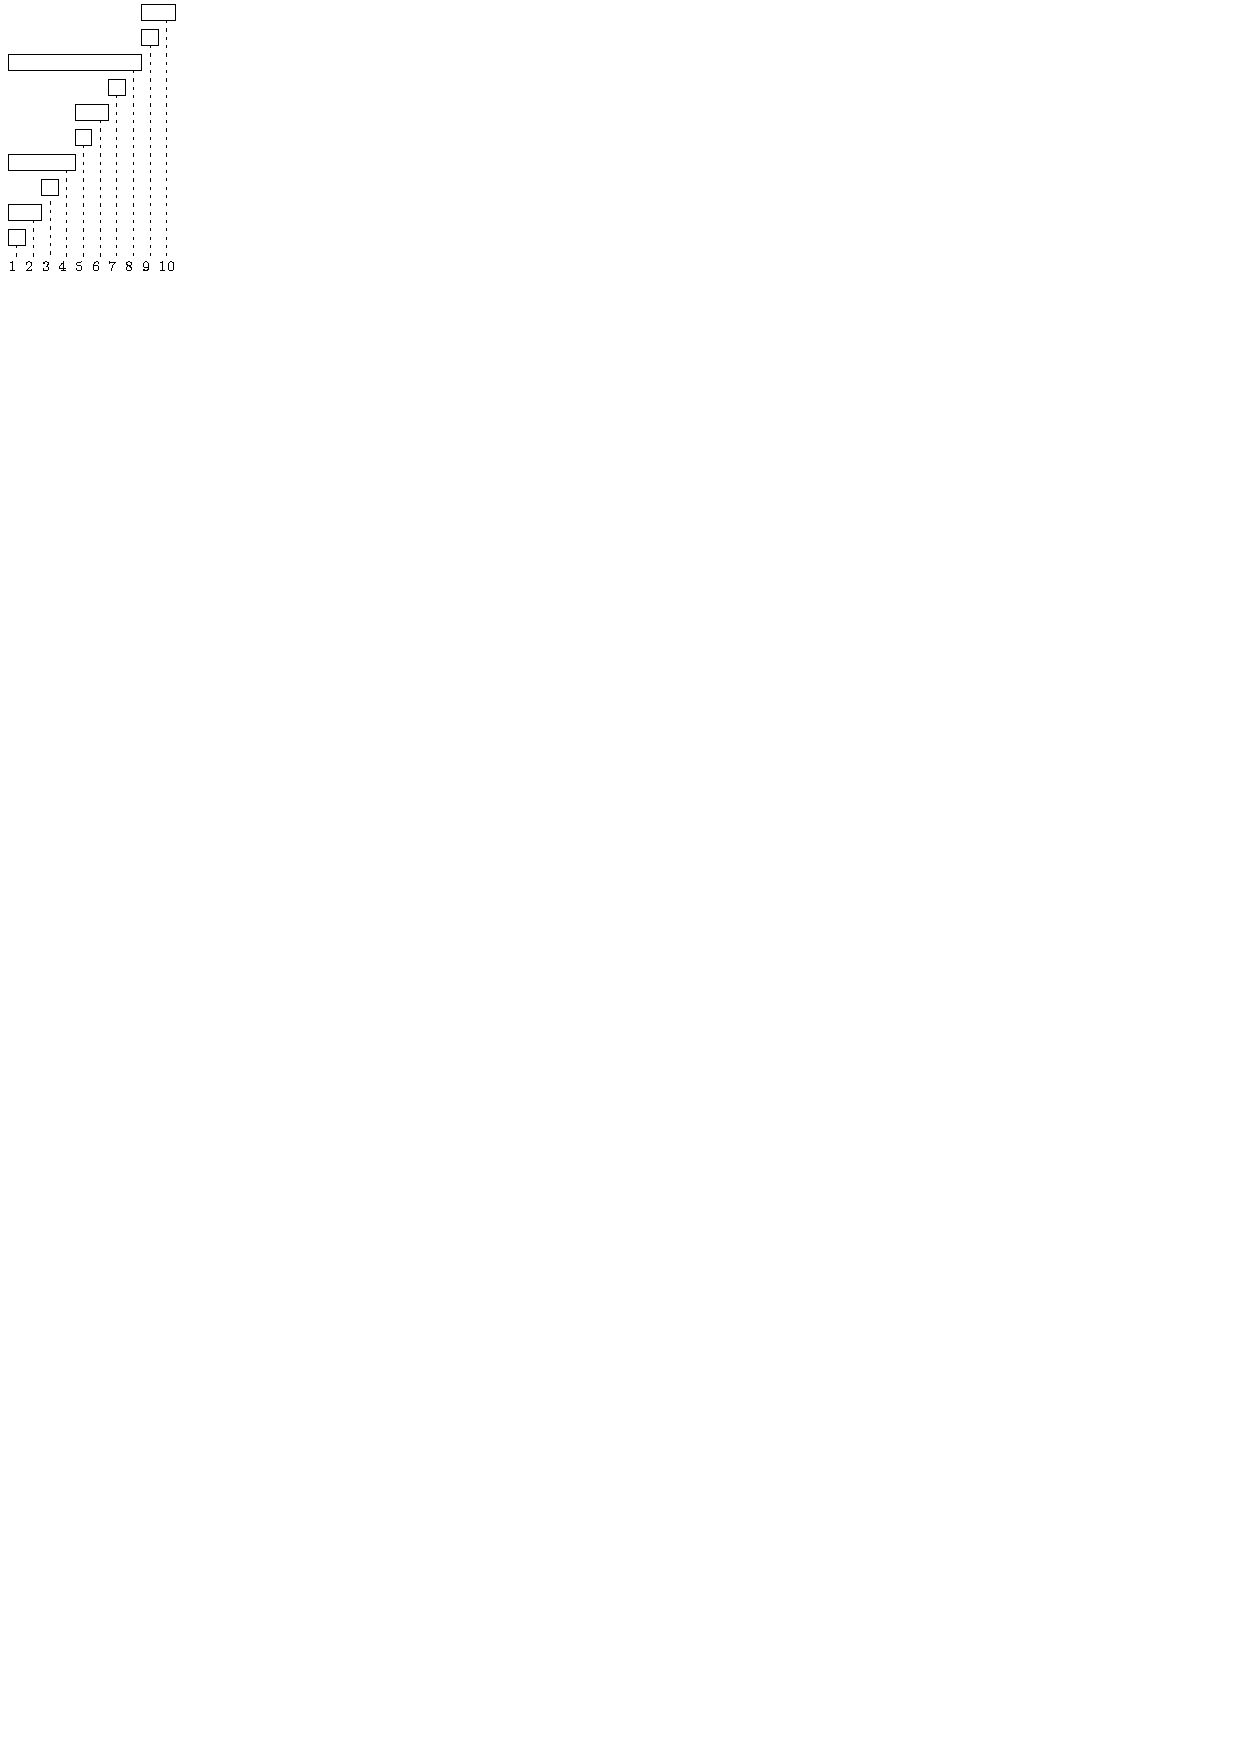
\includegraphics{imgs/bit}
%    \caption{}
%    \label{fig:}
\end{figure}

\begin{tcolorbox}
  对于两个下标 $i$,$j$($i < j$),$B_i$对应的段要么包含在 $B_j$ 对应的段里,要么 $B_i$ 对应的段和 $B_j$ 对应的段不相交。
\end{tcolorbox}


你能证明这个结论吗?

\end{frame}


\begin{frame}{数列$B$的特点}

\end{frame}


\begin{frame}{哪些 $B_j$ 含有 $A_i$}

$B_i$ 是数列 $A$ 里以 $A_i$ 结尾含有 $\lb(i)$ 项的那一段之和。固定 $A_i$,$B$ 的哪些项对应的段里有 $A_i$?
\begin{itemize}
    \item $B_i$ 里有 $A_i$。
    \item 若 $B_j$ 里有 $A_i$ 则 $j \ge i$。
\end{itemize}

对于 $j > i$,若要 $B_j$ 里有 $A_i$,$j$ 要满足什么条件?只要满足

\begin{equation}
    j - \lb(j) < i \label{eq:1}
\end{equation}

\begin{block}{什么样的 $j$ 满足 $\eqref{eq:1}$?}
  既然 $j > i$,设 $j$ 比 $i$ 大的最高位是第 $k$ 位,
 即在第$k$位之前 $j$ 和 $i$ 都相等,在第 $k$ 位上 $j$ 是 $1$而$i$ 是$0$。第一个必要条件是
 \[\lb(j) = k\]
若不然就有 $\lb(j) < k$,$j - \lb(j)$ 仍大于 $i$。
\end{block}

\end{frame}


\begin{frame}{}
第二个必要条件是
\[k > \lb(i)\]
若不然就有  $k < \lb(i)$,则$j - \lb(j) = i$。
上述两必要条件合起来就是充分条件。
\begin{tcolorbox}
  \begin{itemize}
      \item $\lb(j) > \lb(i)$
      \item 在 $\lb(j)$ 之前的位上 $j$ 和 $i$ 相等,在$\lb(j)$ 对应的位上 $j$ 是 $1$,$i$ 是$0$。
  \end{itemize}
\end{tcolorbox}
以 $i = 1010_2$ 为例,$j > i$ 且 $B_j$ 里有 $A_i$ 的下标 $j$ 有 $1100_2, 10000_2, 100000_2, \dots$。
\end{frame}

\end{document}